% !TEX program = xelatex
\documentclass[usenames,dvipsnames]{beamer}
\usefonttheme{serif}
\usefonttheme{structuresmallcapsserif}
\usetheme{Warsaw}
\setbeamertemplate{headline}{} % This line removes the headline template
\usepackage{xcolor}
\beamertemplatenavigationsymbolsempty
\usepackage{tikz}
\usepackage{pgfplots}
\renewcommand{\qed}{\hfill\blacksquare}
\newcommand{\D}[1]{\Delta #1}
\renewcommand{\a}{\alpha}
\usepackage{float}
\newcommand{\heart}{\ensuremath\heartsuit}
\usepackage{todonotes}
\setbeamertemplate{frametitle continuation}{%
    \ifnum\insertcontinuationcount>999999999 % this command tells the program when to start counting and also the count will be in numbers and not in roman letters
    \insertcontinuationcount
    \fi}
% ============================================================ %
% HEBREW support via polyglossia %
% ============================================================ %
\usepackage{polyglossia}
\defaultfontfeatures{Mapping=tex-text, Scale=MatchLowercase}
\setdefaultlanguage{hebrew}
\setotherlanguage{english}
\newfontfamily\hebrewfont[Script=Hebrew]{Arial}
% Use \begin{hebrew} block of text \end{hebrew} for paragraphs.
% Use \texthebrew{ } and \textenglish{ } for short texts.
% ============================================================ %
\title[]{מודל סחירים לא סחירים}
\author{מתן לבינטוב}
\institute[{{ אב"ג}}]{{ אוניברסיטת בן גוריון בנגב}}
\date{}
\usepackage{bidi}
\begin{document}
\begin{RTL}
\begin{frame}
\titlepage
\end{frame}
\begin{frame}
    \frametitle{תוכן עניינים}
    \tableofcontents
\end{frame}
\section{הקדמה וסימונים}
\begin{frame}
    \frametitle{סימונים (פונקציות יצור ליניאריות)}
    \begin{minipage}[t]{0.6\textwidth}
        \begin{align*}
        L_T &- \text{מועסקים בקסטור סחיר} \\
        L_N &- \text{מועסקים בקסטור בלתי סחיר} \\
        P_T &- \text{מחיר מוצר סחיר} \\
        P_N &- \text{מחיר מוצר בלתי סחיר} \\
        W_T &- \text{שכר בסקטור סחיר} \\
        W_N &- \text{שכר בסקטור בלתי סחיר}
        \end{align*}
    \end{minipage}%
    \begin{minipage}[t]{0.5\textwidth}
        \begin{align*}
        Q_T & -  \text{היצע למוצרים סחירים} \\
        Q_N & -  \text{היצע למוצרים בלתי סחירים} \\
        C_T & -  \text{ביקוש למוצרים סחירים} \\
        C_N & -  \text{ביקוש למוצרים בלתי סחירים} \\
        A_T & -  \text{תפוקה ממוצעת במוצרים סחירים} \\
        A_N & -  \text{תפוקה ממוצעת במוצרים בלתי סחירים}
        \end{align*}
    \end{minipage}

    

\end{frame}
\section{יצור מוצרים והחשבון השוטף}
\begin{frame}[allowframebreaks]
    \frametitle{יצור מוצרים והחשבון השוטף}
    \begin{block}{יצור מוצרים}
        יצור מוצרים סחירים,
        $$Q_T = A_T \times L_T$$
        יצור מוצרים בלתי סחירים,
        $$Q_N = A_N \times L_N$$
    \end{block}

    \begin{alertblock}{שימו \heart}
        לא ניתן לייבא / לייצא מוצרים בלתי סחירים, לכן תמיד חייב להתקיים ,$C_N = Q_N$
    \end{alertblock}
    
    \begin{block}{חשבון שוטף}
        \begin{itemize}
            \item $A$ - איזון בחשבון השוטף  $ NX = 0 \iff C_T=Q_T \quad$
            \item \color{blue}$B$ - עודף בחשבון השוטף  $ NX > 0 \iff C_T<Q_T \quad$
            \item \color{red}$C$ - גרעון בחשבון השוטף  $ NX < 0 \iff C_T>Q_T \quad$
        \end{itemize}
    \end{block}

    \framebreak
    % \missingfigure{{להוסיף פה גרף עם 3 נקודות עליו כמו ברשימות המקוריות}}
    \begin{figure}[ht]
        \centering
        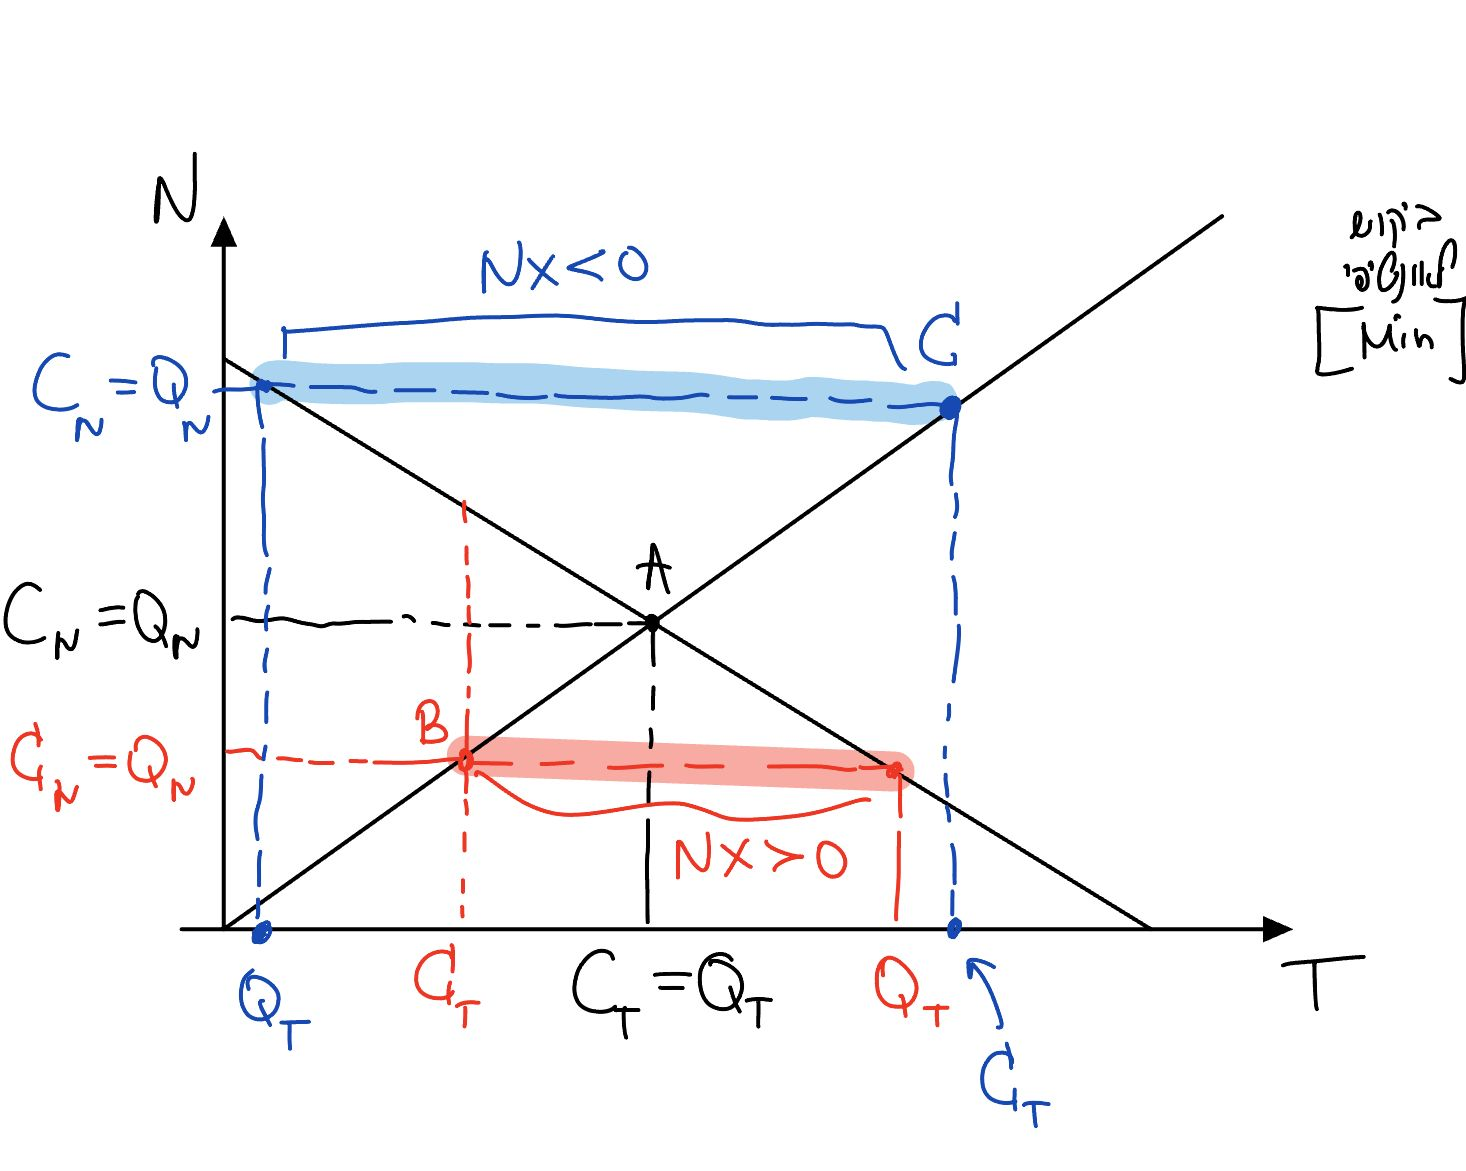
\includegraphics[width=0.9\textwidth]{WhatsApp Image 2024-07-09 at 20.11.28.jpeg}
    \end{figure}
\end{frame}
\section{ביקוש והיצע, מחירים ושכר}
\begin{frame}[allowframebreaks]
    \frametitle{ביקוש והיצע, מחירים ושכר}
    \begin{itemize}
        \item מחיר מוצרים בלתי סחירים נקבע בשוק המקומי בהתאם לביקוש ולהיצע
        \item מחיר מוצרים סחירים נקבע בהתאם לרמת המחירים בעולם
        $$P_T = E \times P_T^{\ *}$$
        \item השכר בסקטור הסחיר והבלתי סחיר נקבע לפי ערך התפוקה שולית פוחתת בכל סקטור,
        $$W_T = A_T \times P_T$$
        $$W_N = A_N \times P_N$$
        \item ניידות מלאה של עובדים בין סקטורים גוררת,
        $$W_T = W_N$$
        \item היצע קשיח של עובדים במשק, 
        $$\bar{L} = L_T + L_N$$
    \end{itemize}
    \framebreak
    \begin{block}{מסקנות}
        באמצעות המשוואה הבאה,
        $$
        W_T = A_T \times P_T = W_N = A_N \times P_N
        $$
        ניתן לדעת מה קרה לשכר ולמחירים היות ו $A_T, P_T, A_N$ הם אקסוגנים, ולכן גם השכר הוא אקסוגני ולכן מה שמשתנה זה מחיר המוצרים הבלתי סחירים. 
       \end{block}
       \begin{block}{מדד המחירים}
        $$P = \alpha \cdot P_T + \left(1- \alpha\right) \cdot P_N$$
       \end{block}
       \begin{block}{שכר ריאלי במשק}
        $$\frac{W}{P} = \frac{W}{\alpha \cdot P_T + \left(1- \alpha\right) \cdot P_N}$$
       \end{block}
\end{frame}

\section{שע''ח ריאלי}
\begin{frame}
    \frametitle{שע''ח ריאלי}
    $$
    e=\frac{E P^*}{P}=\frac{\alpha P_T^*+(1-\alpha) P_N^*}{\alpha P_T+(1-\alpha) P_N}=\frac{\alpha E+(1-\alpha) E \frac{P_N^*}{P_T^*}}{\alpha \frac{P_T}{P_T^*}+(1-\alpha) \frac{P_N}{P_T^*}}=\frac{\alpha+(1-\alpha) \frac{P_N^*}{P_T^*}}{\alpha+(1-\alpha) \frac{P_N}{P_T}}
    $$
    
    \begin{itemize}
        \item אם $e > 1$ - המטבע המקומי חלש ביחס לעולמי
        \item אם $e < 1$ - המטבע המקומי חזק ביחס לעולמי
    \end{itemize}

\end{frame}

\section{שני גורמי יצור}
\begin{frame}[allowframebreaks]
    \frametitle{שני גורמי יצור}
    \begin{itemize}
        \item נניח שהתוצר בשני הסקטורים מיוצר על ידי הון ועבודה
        \item פונקציית היצור בכל ענף היא בעלת תפוקה שולית פוחתת
        \item כמות ההון קבועה
    \end{itemize}
    משמע, בגלל שכמות ההון קבועה ויש תפוקה שולית פוחתת, בעצם יש לנו פונקציית יצור עם תפוקה יורדת לגודל.
    $$
    Q_T = F(L_T, \bar{K_T}), \quad Q_N = F(L_N, \bar{K_N})
    $$
    \begin{itemize}
    \item השיפוע של עקומת התמורה הוא $RPT = \frac{MPL_N}{MPL_T} = \frac{P_T}{P_N}$
    \end{itemize}

    \framebreak
    \begin{figure}[ht]
        \centering
        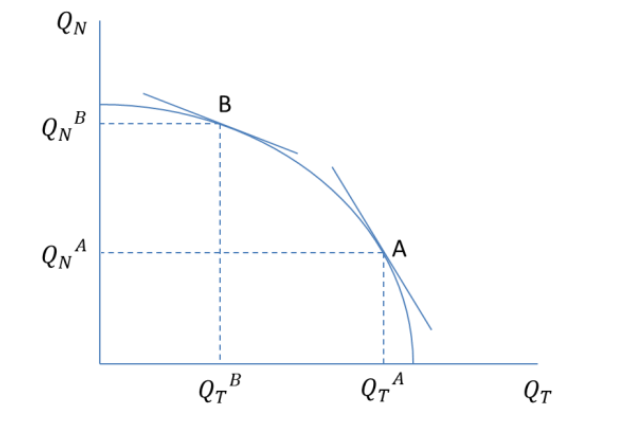
\includegraphics[width=0.8\textwidth]{TNT.png}
    \end{figure}
        \begin{center}
 $Q_T \downarrow \implies L_T \downarrow \implies MPL_T \uparrow \implies W_T \uparrow$
 $Q_N \uparrow \implies L_N \uparrow \implies MPL_N \downarrow \implies W_N \downarrow$
    \end{center}




    
\end{frame}

\section{שיפור טכנולוגי}
\begin{frame}[allowframebreaks]
    \frametitle{שיפור טכנולוגי}
    כאשר יש שיפור טכנלוגי בייצור של מוצרים סחירים אז הייצור של המוצרים עולה
    \begin{figure}[ht]
        \centering
        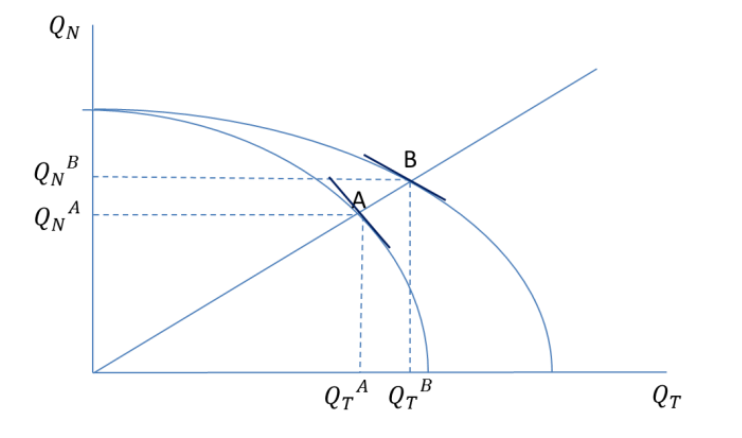
\includegraphics[width=0.6\textwidth]{TNT2.png}

    \end{figure}
$$Q_T \uparrow, L_T \downarrow \implies MPL_T \uparrow \implies W_T \uparrow $$
$$Q_N \uparrow \implies L_N \uparrow \implies MPL_N \downarrow \implies P_N \uparrow \iff W_T \uparrow =  P_N \uparrow \cdot MPL_N \downarrow$$
$$ \downarrow e = \frac{E \cdot P^{\ *}}{P \uparrow}$$
\framebreak
\begin{alertblock}{שימו \heart}
    $$W_T \uparrow =  P_N \uparrow \cdot MPL_N \downarrow$$
    נשים לב שהשכר חייב לעלות (בגלל שהשכר בשוק הסחירים עלה), אבל הגיעו עוד עובדים לשוק הלא סחירים ולכן כדי שהשכר יעלה המחיר של המוצרים הבלתי סחירים חייב לעלות ביותר. \\ 
    מכאן מגיע החשש שרמת המחירים הכוללת במשק עלתה ביותר מהשכר הנומינלי ולכן השכר הראילי נפגע, אך זה תלוי ב $1 - \alpha$, משקל המוצרים הבלתי סחירים במדד המחירים.
\end{alertblock}
\end{frame}

\section{המחלה הולנדית}
\begin{frame}[allowframebreaks]
    \frametitle{המחלה הולנדית}
    כאשר במשק מתגלה אוצר טבע (מוצר סחיר) כמו : נפט או גז הוא מתווסף לייצור המוצרים הסחירים.
    המשק מגדיל את הייצור שלו ב-2 סוגי המוצרים.
    \begin{itemize}
        \item נוצר ייסוף ריאלי שפוגע בענפים הסחירים
        \item נוצר מעבר של עובדים מסקטור סחיר לסקטור הבלתי סחיר, דבר אשר יוצר אבטלה חיכוכית
        \item משום שמשאב הטבע נגמר בסופו של דבר, או שמחירו יורד נוצר קיטון בייצור המוצרים הסחירים. העובדים רוצים לחזור למקומות העבודה הקודמים שלהם, אך לפעמים הם כבר לא קיימים או
        שהעובדים כבר לא בעלי הכשרה מתאימה.
    \end{itemize}
    \framebreak
    \begin{exampleblock}{כיצד מונעים את המחלה}
        אם המשק היה מייצא את כל מה שהוא מפיק, הוא היה יכול להישאר בנקודה $A$ על גבי עקומת
התמורה המקורית. בו זמנית, כדי למנוע ייסוף של המטבע המקומי כתוצאה מהכנסות מט"ח
ממכירת אוצר הטבע, הבנק המרכזי יכול להתערב בשוק המט"ח ולספוג את העודף תוך כדי עיקור
כדי להימנע משינוי כמות הכסף.
    \end{exampleblock}
    \begin{figure}[ht]
        \centering
        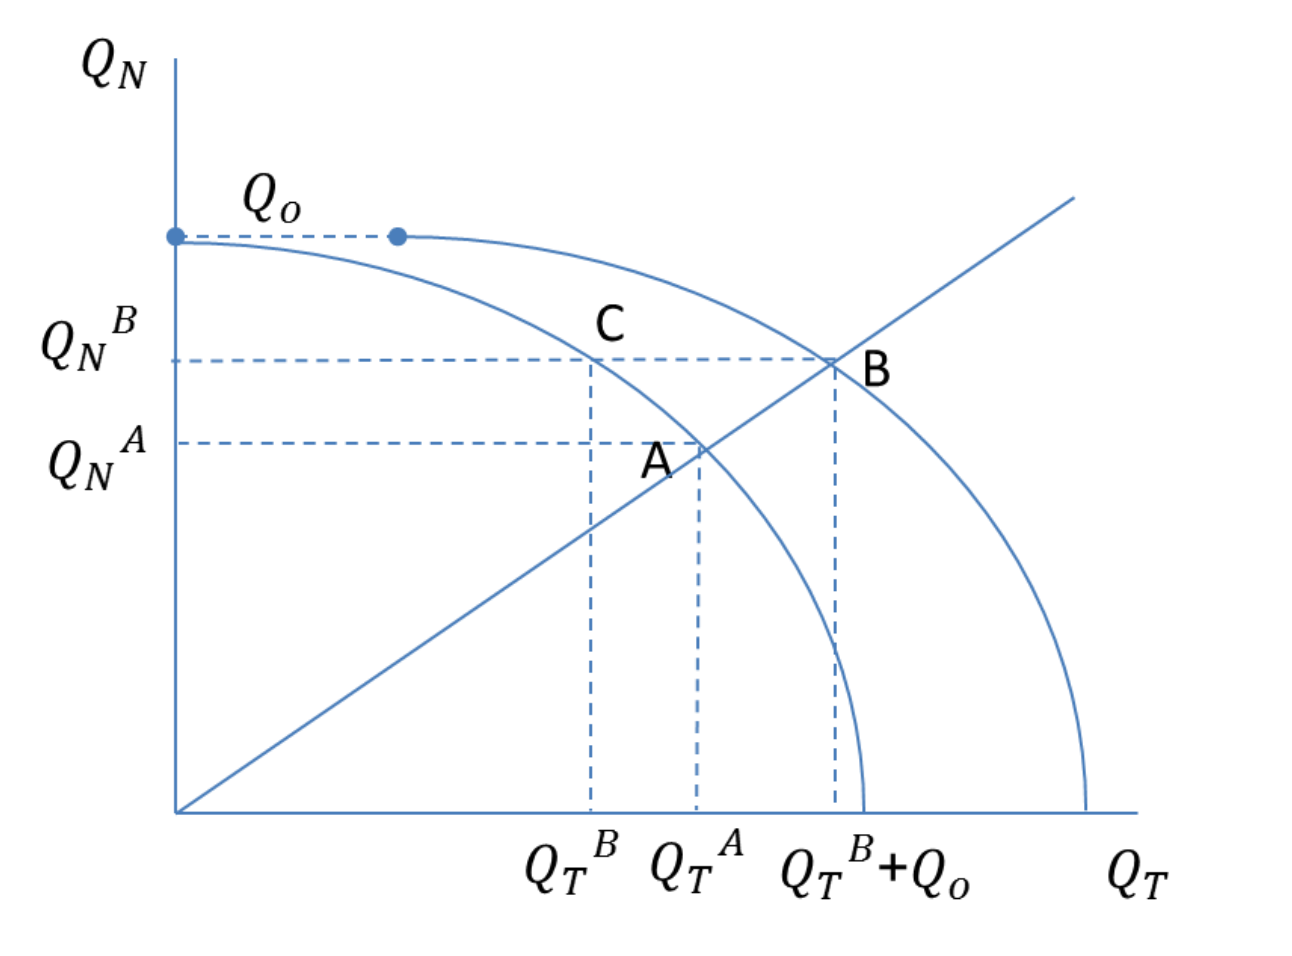
\includegraphics[width=0.6\textwidth]{TNT3.png}

    \end{figure}
\end{frame}
\end{RTL}
\end{document}